\subsection{Introduction}
AlphaGo Zero represents a groundbreaking advancement in artificial intelligence
and reinforcement learning. Unlike its predecessor, AlphaGo, which relied on
human gameplay data for training, AlphaGo Zero learns entirely from self-play,
employing deep neural networks and Monte Carlo Tree Search (MCTS). \cite{agz1}
\\\\ By starting with only the rules of the game and leveraging reinforcement
learning, AlphaGo Zero achieved superhuman performance in Go, defeating the
previous version of AlphaGo in a 100-0 match.
\subsection{Key Innovations}

AlphaGo Zero introduced several groundbreaking advancements over its
predecessor, AlphaGo, streamlining and enhancing its architecture and training
process:

\begin{enumerate}
    \item Unified Neural Network \( f_\theta \): AlphaGo Zero replaced AlphaGo's
          dual-network setup—separate networks for policy and value—with a single neural
          network \( f_\theta \). This network outputs both the policy vector \( p \) and
          the value scalar \( v \) for a given game state, reprsented as

          \begin{equation}
              f_\theta(s) = (p, v)
          \end{equation}

          This unified architecture simplifies the model and improves training
          efficiency.

    \item Self-Play Training: Unlike AlphaGo, which relied on human games as training
          data, AlphaGo Zero was trained entirely through self-play. Starting from random
          moves, it learned by iteratively playing against itself, generating data and
          refining \( f_\theta \) without any prior knowledge of human strategies. This
          removed biases inherent in human gameplay and allowed AlphaGo Zero to discover
          novel and highly effective strategies.

    \item Removal of Rollouts: AlphaGo Zero eliminated the need for rollouts, which were
          computationally expensive simulations to the end of the game used by AlphaGo's
          MCTS. Instead, \( f_\theta \) directly predicts the value \( v \) of a state,
          providing a more efficient and accurate estimation.

    \item Superior Performance: By integrating these advancements, AlphaGo Zero defeated
          AlphaGo 100-0 in direct matches, demonstrating the superiority of its self-play
          training, unified architecture, and reliance on raw rules over pre-trained
          human data.
\end{enumerate}

\subsection{Training Process}

\subsubsection{Monte Carlo Tree Search (MCTS) as policy evaluation operator}
Intially the neural network \( f_\theta \) is not very accurate in predicting
the best move, as it is intiallised with random weights at first. To overcome
this, AlphaGo Zero uses MCTS to explore the game tree and improve the policy.
\\\\ At a given state S, MCTS expands simualtions of the best moved that are
most likely to generate a win based on the initial policy $P(s,a)$ and the
value $V$. MCTS iteratively selects moves that maximize the upper confidence
bound (UCB) of the action value. UCB is designed to balanced exploration and
exploitation. and it is defined as

\begin{equation}
    UCB = Q(s, a) + U(s, a)
\end{equation}

where \[U(s, a) \propto \frac{p(s, a)}{1 + N(s, a)}\] MCTS at the end of the search returns the policy vector \( \pi \) which is used
to update the neural network \( f_\theta \) by minimizing the cross-entropy
loss between the predicted policy by $f_\theta$ and the MCTS policy.

\subsubsection{Policy Iteration and self play}
The agent plays games against itself using the predicted policy $P(s, a)$. The
agent uses the MCTS to select the best move at each state and the game is
played till the end in a process called self play. The agent then uses the
outcome of the game, $z$ game winner and $\pi$ to update the neural network.
This process is repeated for a large number of iterations.

\subsubsection{Network Training Process}

The neural network is updated after each self-play game by using the data
collected during the game. This process involves several key steps:
\begin{enumerate}
    \item Intilisation of the network: The neural network starts with random weights
          $\theta_0$, as there is no prior knowledge about the game.
    \item Generating Self-play Games: For each iteration $i \geq 1$ self-play games are
          generated. During the game, the neural network uses its current parameters
          $\theta_{i - 1}$ to run MCTS and generate search probabilities $\pi_t$ for each
          move at time step $t$.
    \item Game Termination and scoring: A game ends when either both players pass, a
          resignation threshold is met, or the game exceeds a maximum length. The winner
          of the game is determined, and the final result $z_t$ is recorded, providing
          feedback to the model.
    \item Data Colletion: for each time step $t$, the training data $(s_t, \pi_t, z_t)$
          is stored, where $s_t$ is the game state, $\pi_t$ is the search probabilities,
          and $z_t$ is the game outcome.
    \item Network training process: after collecing data from self-play, The neural
          network $f_\theta$ is adjusted to minimize the error between the predicted
          value v and the self-play winnder z, and to maximize the similarity between the
          search probabilities $P$ and the MCTS probabilities. This is done by using a
          loss function that combines the mean-squared error and the cross entropy losses
          repsectibly. The loss function is defined as

          \begin{equation}
              L = (z - v)^2 - \pi^T \log p + c||\theta||^2
          \end{equation}

          where $c$ is the L2 regularization term.

\end{enumerate}

\subsection{Challenges and Solutions}
Alpha Go Zero overcame several challanges:
\begin{enumerate}
    \item Human knowledge Dependency: AlphaGo Zero eliminated the need for human gameplay
          data, relying solely on self-play to learn the game of Go. This allowed it to
          discover novel strategies that surpassed human expertise.
    \item Compelxity of the dual network approach in alpha go: AlphaGo utilized separate
          neural networks for policy prediction $p$ and value estimation $V$, increasing
          the computational complexity. AlphaGo Zero unified these into a \textbf{single
              network} that outputs both $p$ and $V$, simplifying the architecture and
          improving training efficiency.
    \item The need of handcrafted features: AlphaGo relied on handcrafted features, such
          as board symmetry and pre-defined game heuristics, for feature extraction.
          AlphaGo Zero eliminated the need for feature engineering by using \textbf{raw
              board states} as input, learning representations directly from the data.
\end{enumerate}

\subsection{Performance Benchmarks}

AlphaGo Zero introduced a significant improvement in neural network
architecture by employing a unified residual network (ResNet) design for its
$f_\theta$ model. This replaced the separate CNN-based architectures previously
used in AlphaGo, which consisted of distinct networks for policy prediction and
value estimation. \\\\ The superiority of this approach is evident in the Elo
rating comparison shown in figure \ref{fig:results_agz}. The "dual-res"
architecture, utilized in AlphaGo Zero, achieved the highest Elo rating,
significantly outperforming other architectures like "dual-conv" and "sep-conv"
used in earlier versions of AlphaGo.

\begin{figure}[ht]
    \centering
    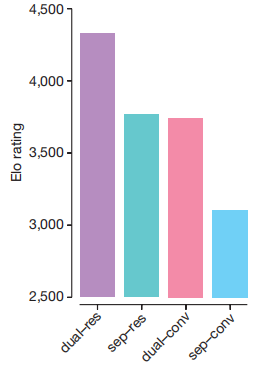
\includegraphics[width=0.20\textwidth]{sections/5AlphaGo Zero/Results_agz.png}
    \caption{Elo rating comparison of different neural network architectures.}
    \label{fig:results_agz}
\end{figure}

